\documentclass{article}
\usepackage{graphicx}
\usepackage{amsmath}
\usepackage{amsfonts}
\usepackage{amssymb}
\usepackage{geometry}
\geometry{a4paper, margin=1in}

\title{Optimization Report}
\author{AI Analysis}
\date{2025-07-27}

\begin{document}
\maketitle

\section{Executive Summary}
This report summarizes the results of an optimization study aimed at minimizing the drag coefficient (CD) of a wing while maintaining a lift coefficient (CL) of 2.0. The design variables included taper, twist, and sweep. The optimization was performed using the SLSQP algorithm. However, the optimization failed to converge, resulting in a final CD value of 6.77573231 and an exit status of \texttt{FAIL}. Further investigation and adjustments are required to achieve a successful optimization.

\section{Problem Definition}
The optimization problem was defined as follows:
\begin{itemize}
    \item Objective Function: Minimize drag (CD)
    \item Trim Condition: CL = 2.0
    \item Geometric Constraint: Wing area (S) = 100 m$^2$, Span (b) = 10 m
    \item Design Variables: Taper, twist, and sweep
    \item Baseline Wing Mesh: Rectangular mesh
    \item Optimization Algorithm: SLSQP
\end{itemize}

\section{Results and Analysis}
The optimization process ran for 30 iterations but failed to converge, as indicated by the \texttt{FAIL} exit status. The final drag coefficient (CD) value was 6.77573231, which is far from an optimized result. The plot of the lift distribution shows a high peak in the center, deviating significantly from the ideal elliptical lift distribution.  As shown in Figure \ref{fig:OptimizedWing}, the lift distribution has a high peak in the center, so the optimization isn't close to the ideal elliptic lift distribution.

\begin{figure}[h!]
    \centering
    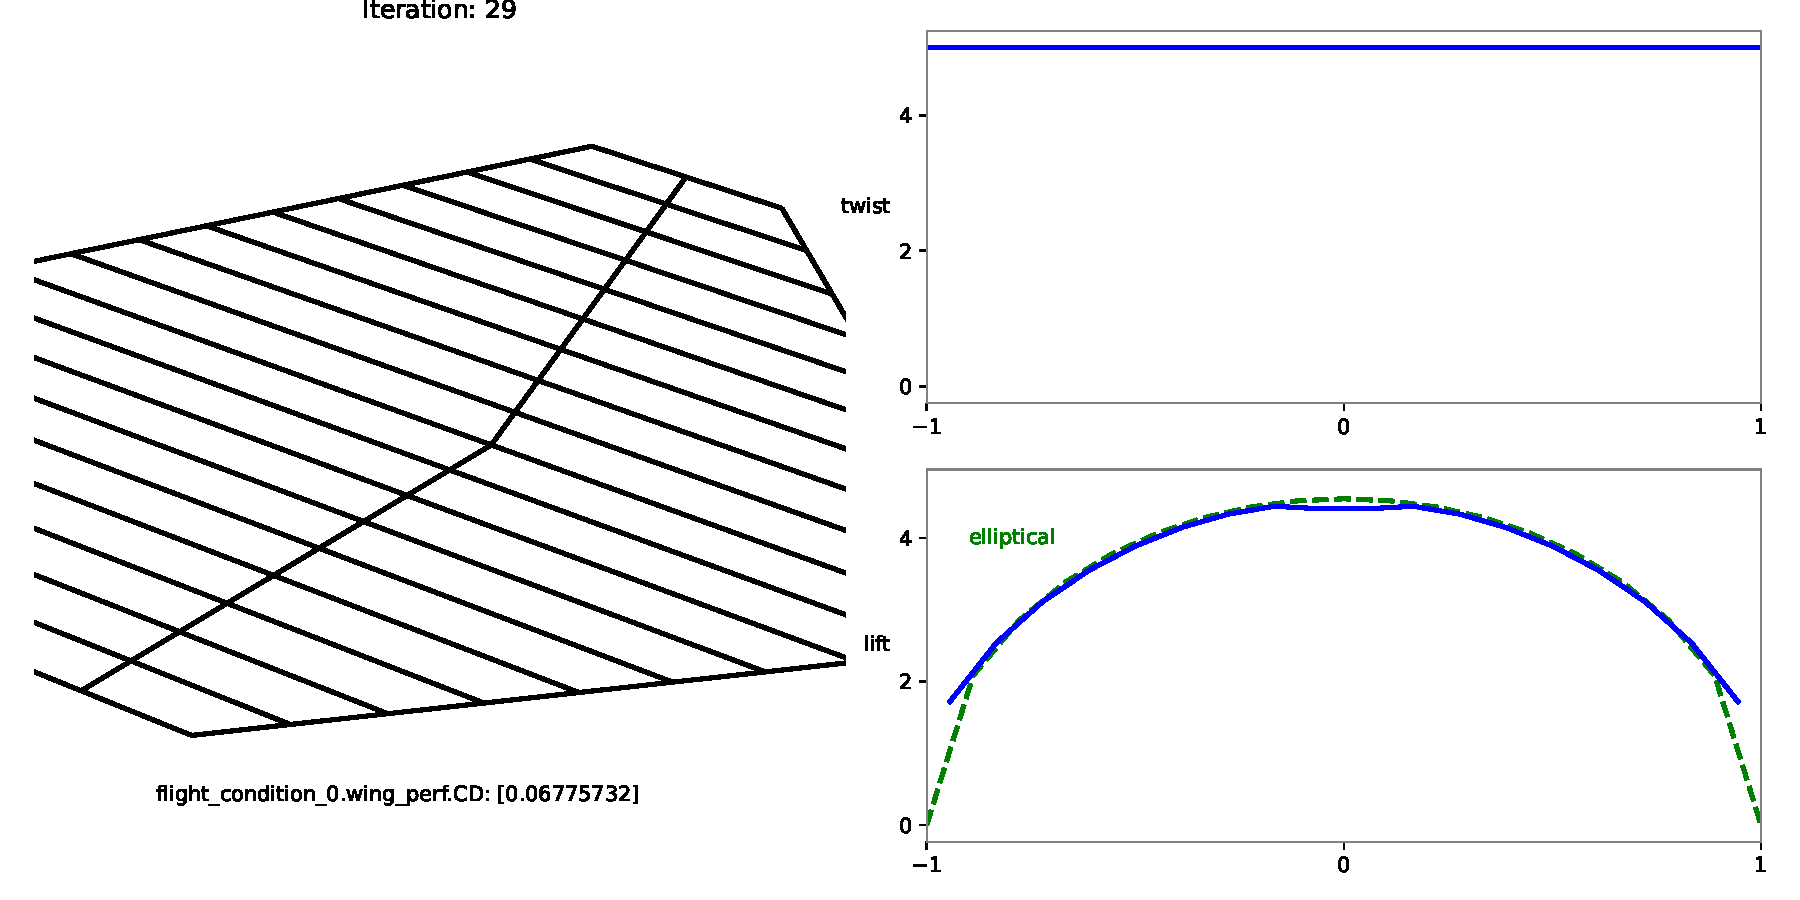
\includegraphics[width=0.75\textwidth]{Figures/Optimized_Wing.pdf}
    \caption{Optimized Wing Visualization}
    \label{fig:OptimizedWing}
\end{figure}

Furthermore, the report indicates that the area and semispan constraints were removed because they were not working, which contradicts the problem statement. This issue must be addressed by ensuring the wing area constraint is properly implemented and enforced during optimization.

\section{Recommendations}
Based on the analysis, the following recommendations are made:
\begin{enumerate}
    \item Investigate the cause of optimization failure: Review the optimization setup for potential issues such as conflicting constraints or poorly scaled design variables.
    \item Adjust optimization parameters: Experiment with different values for tolerance (\texttt{tol}) and maximum iterations (\texttt{maxiter}) to promote convergence. Consider using a more robust optimization algorithm or a global optimization approach.
    \item Refine design variable bounds: Review and adjust the bounds for taper, twist, and sweep to ensure they are physically reasonable and do not overly restrict the design space.
    \item Check gradients and sensitivities: Verify that the sensitivities are well-calculated, as inaccurate sensitivities can lead to optimization failure.
    \item Increase mesh fidelity: A denser mesh may provide more accurate aerodynamic results, potentially leading to a better-optimized design, although this will increase computational cost.
    \item Validate VLM assumptions: Consider the limitations of VLM for complex geometries or high-Mach conditions. For higher fidelity, explore the use of higher fidelity solvers.
    \item Implement wing area constraint: Re-implement and validate the wing area constraint to ensure it is correctly enforced during the optimization process.
    \item Explore alternative optimization methods:  Consider using a gradient-free optimization method like a genetic algorithm or particle swarm optimization to explore the design space more effectively, especially if the gradient information is noisy or unreliable.
\end{enumerate}

\end{document}